%%%%%%%%%%%%%%%%%%%%%%%%%%%%%%%%%%%%%%%%%%%%%%%%%%%%%%%%%%%%%%%%%%%%%%%%%%%%%%
%%%%%%%%%%%%%%%%%%%%%%%%%%%%%%%%%%%%%%%%%%%%%%%%%%%%%%%%%%%%%%%%%%%%%%%%%%%%%%
%%
%% Dokumentacia k projektu z ZZN
%%
%%%%%%%%%%%%%%%%%%%%%%%%%%%%%%%%%%%%%%%%%%%%%%%%%%%%%%%%%%%%%%%%%%%%%%%%%%%%%%
%%%%%%%%%%%%%%%%%%%%%%%%%%%%%%%%%%%%%%%%%%%%%%%%%%%%%%%%%%%%%%%%%%%%%%%%%%%%%%
\documentclass[12pt,a4paper,titlepage,final]{article}

% cestina a fonty
\usepackage[czech]{babel}
\usepackage[utf8]{inputenc}
% balicky pro odkazy
\usepackage[bookmarksopen,colorlinks,plainpages=false,urlcolor=blue,unicode]{hyperref}
\usepackage{url}
% obrazky
\usepackage[dvipdf]{graphicx}
% velikost stranky
\usepackage[top=3.5cm, left=2.5cm, text={17cm, 24cm}, ignorefoot]{geometry}

\begin{document}

%%%%%%%%%%%%%%%%%%%%%%%%%%%%%%%%%%%%%%%%%%%%%%%%%%%%%%%%%%%%%%%%%%%%%%%%%%%%%%
% titulná strana

% !!!!!!!!!!!!!!!!!!!!!!!!!!!!!!!!!!!!!!!!!!!!!!!!!
\def\author{Martin Maga}
\def\email{xmagam00@stud.fit.vutbr.cz}
\def\projname{Riešenie \\Projekt z predmetu SIN \\  \Large{Zadanie: Dopravní telematika} }
% !!!!!!!!!!!!!!!!!!!!!!!!!!!!!!!!!!!!!!!!!!!!!!!!!

\begin{titlepage}

% \vspace*{1cm}
\begin{figure}[!h]
  \centering
  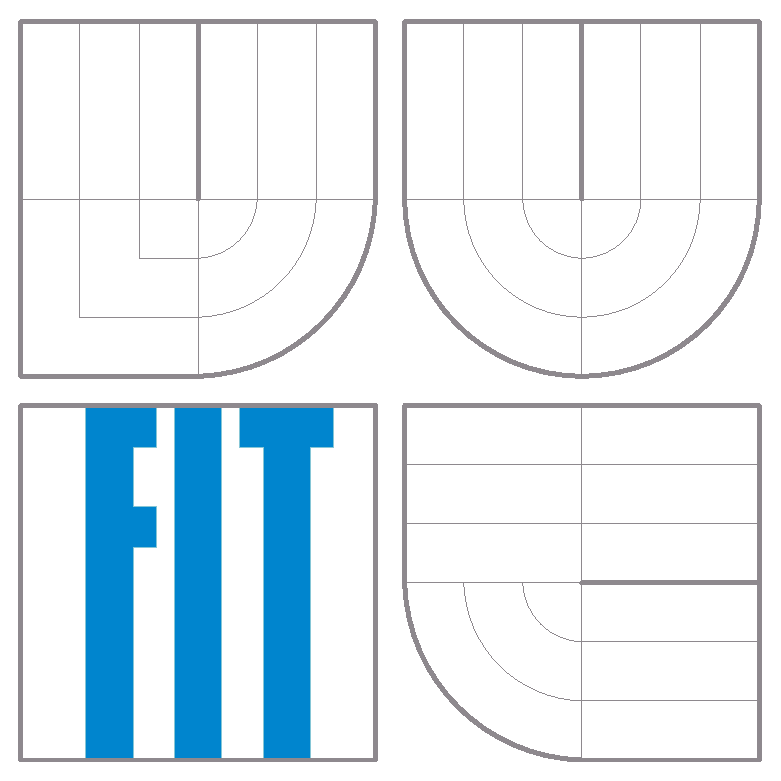
\includegraphics[scale = 0.6]{img/logo.eps}
\end{figure}

\vfill

\begin{center}
\begin{Large}

\end{Large}
\bigskip
\begin{Huge}
\projname\\
\end{Huge}
\begin{large}

\end{large}
\end{center}

\vfill

\begin{center}
\begin{Large}
\today
\end{Large}
\end{center}

\vfill

\begin{flushleft}
\begin{large}
\begin{tabular}{ll}
Autor: Martin Maga (xmagam00), Vojtěch Meca (xmecav00) - vedúci tímu, \\              
  Fakulta Informačních Technologií \\
  Vysoké Učení Technické v~Brně \\
\end{tabular}
\end{large}
\end{flushleft}
\end{titlepage}

\tableofcontents
\newpage

\section{Riešenie}

\subsection{Zadání}
Zadanie spočíva v tvorbe modelu križovatky v nami zvolenom simulačnom frameworku. Cieľom je model križovatky, ktorý bude riešiť problematiku dopravnej telekinematiky tj možné problémy a riešenie, ktoré by mohlo riešiť problémy z praxe.

\section{Návrh a cieľ riešenia}
Cieľom projektu je automatizácia križovatky. Uvažujeme jednoduchú križovatku so štyrmi smermi SEVER, JUH, VÝCHOD A ZÁPAD. Činnosť križovatky nei je závislá na nejakej časovej perióde tj. križovatka je prevádzka cez deň aj v noci. Počas simulácia sbierame štatistiky príchodu aút, ktoré sú náhodné generované v každom smere, rovnako aj stav semaforom a počet aút pred jednotlivými semaformi, tj vo frontách.

\section{Implementácia}
Projekt je implementovaný v Jave s využitím simulačného frameworku JADE, čo je platforma založená na jazyku Java.

Jadro projektu tvorí model križovatky v tvare X a križovatka obsahuje 2 semafory, pričom autá prichádzajú v každom smere.

Beh modelu je založený na náhodnom generovaní aút v každom smere, pričom pred každým semaforom sa tvorí istá fronta, ktorá má svoju maximálnu dĺžku. Semafory sú riadené stochatiským procesom, pričom každý semafor má informáciu o tom koľko aút aktuálne pred ním čaká. Tieto informácie sa používajú k vyhodnoteniu situácie a spusteniu smerom, v ktorom je väčší počet aút. 

V projekte je striktne dodržaná agentná architektúra, ktorá znamená, že jednotlivý agenti sú vzájomne nezávislí a komunikujú prostredníctvom zvolených správ.

CreatorAgent predstavuje hlavného agenta, ktorý obsluhuje aj ostatných agentov. Tento agent je zodpovedný za spustenie behu celej aplikácie a generovanie aút pre každý semafor (agenta). Zároveň pri generovaní posiela informácie o nagenerovaných autách jednotlivým agentom. Títo agenti (RouteAgent) spracovávajú prijáte správy o pridaní nových aút a posielajú informácie späť hlavnému agentovi. Hlavný agent (CreatorAgent) podľa prijatých informácií od jednotlivých agentov rozhoduje, ktorí semafor bude mať zelenú a ktorý červenú. Zároveň prebieha logovanie na úrovni konzole, kde sú zobrazované stavové a súhrné informácie o autách a aktuálnom stave semaforov.

\newpage
\section{Štatistiky križovatky}
Hlavným cieľom aplikácie je okrem funkčnosti je poskytnúť aktuálnu situáciu o stave frontách pre jednotlivé semafory (agentov). Do konzole sa pravidelne zobrazujú informácie nasledovného formátu: 

\begin{equation} 
  nazovangeta-stavSemaforu-"smer-1.auto-veľkost fronty-smer-1.auto-veľkost fronty
\end{equation}

Príklad:

\begin{equation} 
  route1-GREEN-N-2-3-S-4-5
\end{equation}

Vyššie uvedený príklad odpovedá výstupu fronty pre 1. agenta obsluhujúci semafor zo severu a juhu križovatky. Pričom vieme povedať, že 1. auto na križovatke zo severu má ID 2 a na semafore čakajú celkovo 3 autá a z má 1. auto na semafore ID 4 a na semafore čaká celkovo 5 aút. Všetky tieto správy sú spracované zároveň hlavným agentom (CreatorAgent), ktorý tieto správy rozparsuje a rozhodne činnosti križovatky, tj v ktorých smeroch budú pustené autá.

\section{Agenti}
\begin{itemize}
\item CreatorAgent - Hlavný agent, ktorý sa stará o spustenie celého modelu a zároveň generovanie aút a zároveň prijíma správy od agentov na semaforoch a rozhoduje, ktoré semafory budú pustené
\item RouteAgent - Agent, ktorý prijíma správy od Creator agenta zaraďuje autá do jednotlivých interných front a stavu front sa posielajú CreatorAgent-ovi
\end{itemize}

\newpage
\section{Rozšírenia}
Aplikácia obsahuje len konzolový výstup, ktorý je trochu obmedzujúci. Preto ako možné rozšírenie môže aplikácia obsahovať GUI, ktoré bude zbierať štatistické výstupy a vykreslovaŤ GUI. Teda bude obsahovať semafory, autá pred semaformi. 

Ďalšie možné rozšírenie môže predstavovať striedanie dňa a noci, ktorý by mohlo byť realizované ďalším agentom, ktorý bude informovať ostatných agentov. Toto bude mať za následok, že počas dňa budú semafory pustené a počas noci budú vypnuté.

Rovnako by náš model mohol obsahovať viac prijázdových pruhov pred semaformi, ktoré by bolo následne obsluhované agentom na semafore.

Rovnako by semafor, v prípade, že by aplikácia bola vybavená GUI zobrazovať počet aút, ktoré križovatkou prejdu a spôsob rozhodovania.

Rovnako by užívateľ mohol sám v nejakom formáte vložiť vlastné pravidlá, ktoré by mohli ovplyvňovať celkové ovládanie križovatky.




\newpage
\section{Záver}
Poradilo sa nám vytvoriť správny a korektný model simulujúci križovatku. Modal obsahuje niekoľko semaforov, pričom pred každým semaforom sa tvorí fronta aút, pričom autá do tejto fronty sú náhodne generované a následne sú autá zaraďované do front. Vizualizácia prebieha zapisovaním správ do konzole. Možné vylepšenie predstavuje tvorba GUI pre lepšiu vizualizáciu stavu križovatky. 

V projekte sme dodržali agentnú architektúru. Agenti nie sú na sebe závislí a nemajú pevné väzby a komunikácia prebieha prostredníctvom správ.

\end{document}

